\chapter{Vergleich der Annotationen für die Implementierung}

Nachdem bereits die Spezifikationen und darin verwendete Sprachmittel verglichen wurden,
behandelt dieses Kapitel nun die Verifizierung der Implementierungen.
Die Werkzeuge VeriFast bzw. Frama-C führen dazu eigene Berechnungen durch, benötigen aber dennoch
zusätzliche Annotationen im Quellcode, damit die korrekten logische Schlüsse gezogen 
werden können. Beispielsweise muss der Code um Schleifeninvarianten oder 
Ghost-Befehle ergänzt werden, die Prädikate oder weitere logische Beweise mit einbeziehen.


\section{Symbolische Ausführung in VeriFast}

Die Verifizierung des Implementierungs-Codes findet in VeriFast mit Hilfe einer symbolischen Ausführung statt:
Begonnen wird mit den Vorbedingungen des Methodenvertrags, der Code wird dann wie bei der tatsächlichen
Ausführung vorwärts verarbeitet. Jedoch nicht mit konkreten, sondern mit 
abstrakten Werten. Diese werden durch logische Formeln repräsentiert, welche die möglichen Variablenwerte 
beschreiben. Am Ende der Ausführung sind dann bei erfolgreicher Verifizierung alle Voraussetzungen
erfüllt, um die Nachbedingungen direkt abzuleiten.

\begin{SCfigure}[1.7][h!]
	\centering
		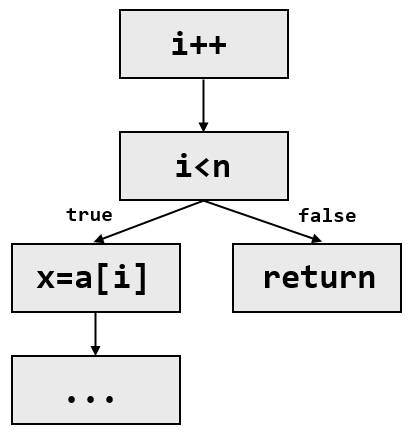
\includegraphics[width=0.3\textwidth]{images/symbolic_execution.png}
		\caption{Ausführungspfade für die symbolische Ausführung einer if-Anweisung}
\end{SCfigure}

Während der symbolischen Ausführung werden alle potenziellen Ausführungspfade untersucht: Schleifen
oder auch \texttt{if}-Anweisungen sorgen dafür, dass VeriFast diese Verzweigungen einzeln betrachtet
und verifiziert. Existieren mehrere \texttt{return}-Anweisungen in der Implementierung, so stellt
das Werkzeug sicher, dass in jedem Ausgang die Nachbedingungen gelten.

Der aktuelle Ausführungszustand setzt sich dabei aus folgenden Elementen zusammen: 
Dem symbolischen Heap zur Verwaltung der Heap-Chunks, dem symbolischen Speicher sowie den Pfadbedingungen
(engl. path conditions) \cite[Kap. 2]{jacobs-2010}. 

Der symbolische Speicher bildet die aktuellen lokalen Variablen auf die entsprechenden logischen Formeln ab.
Die Pfadbedingungen hingegen sind Folgerungen, die aus der Ausführung des Implementations-Codes und aus den Annotationen
berechnet werden. Für den \texttt{false}-Pfad der Verzweigung aus Abbildung 4.1 wird beispielsweise
\lstinline{i >= n} geschlussfolgert.

Zum Verständnis der einzelnen Schritte ist die VeriFast-Oberfläche sehr hilfreich, da sie den aktuellen
Zustand für einen beliebigen Haltepunkt anzeigen kann. Die folgende Situation zeigt die Ausführung
einer \lstinline{mismatch}-Implementierung bis zum gesetzten Haltepunkt (gelb hervorgehoben).

\begin{figure}[ht]
\centering
\includegraphics[width=1.0\textwidth]{images/VeriFast-state-after-precondition.png}
\caption{VeriFast-Oberfläche, symbolische Ausführung bis zum gesetzten Haltepunkt}
\end{figure}

Gut zu erkennen ist, dass logische Ausdrücke wie \(n >= 0\) in die Liste der Pfadbedingungen 
(im Bild als \glqq Assumptions\grqq{} betitelt) aufgenommen wurden. Die \lstinline{ints}-Prädikate hingegen
wurden zum Heap hinzugefügt. Diesen Prozess nennt VeriFast \glqq Producing assertion\grqq, wobei sich das Verb
\glqq Producing\grqq{} auf das Hinzufügen von Elementen zum aktuellen Zustand der symbolischen Ausführung
bezieht.

Das Gegenteil - \glqq Consuming assertion\grqq{} - findet z.B. beim Verifizieren der Nachbedingungen statt.
VeriFast versucht dann alle erforderlichen Aussagen in der Liste der Annahmen bzw. im Heap zu finden
und diese, wenn sie denn passen, zu entfernen. Zusätzlich dazu wird am Ende einer Funktion überprüft, 
dass der Heap (der aktuellen Funktion) leer ist. Ist das nicht der Fall so wurde der entsprechende Speicher 
nicht korrekt bereinigt oder zumindest war VeriFast nicht in der Lage die korrekte Bereinigung zu beweisen.

Im Fall von mismatch würde VeriFast die Heap chunks \lstinline{ints(a, n, al)} sowie
\mbox{\lstinline{ints(b, n, bl)}} beim Konsumieren der Nachbedingung auf dem Heap finden, entfernen und
somit erfolgreich verifizieren können, dass der Speicher so wie vor dem Aufruf vorhanden ist.



\section{Assertions und Ghost-Commands}

Zusicherungen (engl. assertions) und Ghost-Commands sind Annotationen, die direkt in den Implementierungs-Code
eingefügt werden. Assertions stellen sicher, dass der enthaltene Ausdruck wahr ist und sind ein nützliches Hilfsmittel, 
um die Verifizierung besser nachzuvollziehbar und verständlich zu machen. Insbesondere bei 
nicht trivialen Schlussfolgerungen, ist es von Vorteil sie zu ergänzen und im Code zu belassen. Ghost-Commands hingegen 
enthalten Anweisungen für die Verifizierung, z.B. das Verwenden weiterer Definitionen oder Sätze. Sie helfen dem Werkzeug 
beim Ziehen logischer Schlüsse.

Der folgende Quellcode zeigt einen Ausschnitt einer rekursiven Implementierung für \lstinline{equal} und dient
als Anschauungsmaterial für die Erklärung der zwei Annotationstypen:

\lstinputlisting[language=C, caption=Rekursive Implementierung für \lstinline{equal} mit VeriFast]{codes/equal_recursive_VeriFast.c}

Diese Implementierung zeigt nur die Abbruchbedingung der Rekursion -- ist \lstinline{n == 0}, so sind die
leeren Listen gleich und die Berechnung terminiert. 

Die Zeilen 9 und 10 sind Zusicherungen, die formal beschreiben, dass die induktiven Listen \lstinline{al} und
\lstinline{bl} die Länge 0 haben müssen und somit gleich lang sind. Damit VeriFast in der Lage ist das zu
beweisen, sind die zwei Ghost-Commands in Zeile 5 und 6 notwendig. Sie öffnen das \lstinline{ints}-Prädikat
und bringen somit dessen Inhalt in die Liste der Annahmen. Erst dadurch ist für VeriFast ersichtlich, dass 
\lstinline{n} gleichzusetzen ist mit \texttt{length(al)} und \texttt{length(bl)}. Außerdem produziert
das Öffnen des Prädikats die Formel \lstinline{al = nil} bzw. \lstinline{bl = nil} (siehe Definition
des Prädikats in Listing 3.9 oder 4.2). Damit löst sich die Assertion \lstinline{al == bl} in den
trivialen Vergleich \lstinline{nil == nil} auf.

Das Öffnen der Prädikate konsumiert gleichzeitig auch die entsprechenden Heap-Chunks, was jedoch dazu führt,
dass diese beim Produzieren der Nachbedingung fehlen. Sie müssen also vor der \(return\)-Anweisung
wieder geschlossen werden (Zeile 11 und 12), damit sie dann wieder an den Aufrufer zurückgegeben werden können 
- so wie es die Nachbedingung verlangt.

Das Schreiben dieser \texttt{close}-Annotation ist jedoch oft nicht notwendig, da VeriFast sie automatisch
einführt, wenn es sich um ein sogenanntes präzises Prädikat handelt. Darunter versteht VeriFast Prädikate mit 
eingehenden und ausgehenden Parametern, die exakt die gleiche Speicherregion repräsentieren. 

Die Kennzeichnung als präzises Prädikat geschieht über die Nutzung eines Semikolons bei der Trennung
der Prädikaten-Parameter:

\lstinputlisting[language=C, caption=Präzises Prädikat \lstinline{ints}]{codes/ints_precise_predicate_VeriFast.c}

Präzise Prädikate versucht VeriFast während der Verifizierung automatisch zu öffnen und ggf. auch zu
schließen. Dadurch ist in der obigen Implementierung das Schreiben der \texttt{close}-Anweisungen
nicht zwingend notwendig.

Assertions in ACSL werden genauso notiert wie in VeriFast. Ghost-Commands hingegen werden
mit dem Schlüsseltwort \lstinline{ghost} eingeleitet, sind aber generell nicht so oft wie in
VeriFast notwendig. Das kommt daher, dass Frama-C aufwendigere Berechnungen durchführt, um
entsprechende logische Schlüsse zu ziehen. 


\section{Schleifeninvarianten}

Schleifeninvarianten beschreiben eine Eigenschaft, die vor und nach jeder Iteration gültig ist. Sie
werden wie Ghost-Commands per Annotation an die Schleife geschrieben und helfen dem Werkzeug die
Nachbedingungen zu verifizieren.

Der folgende Quellcode zeigt eine ACSL-Implementierung für \lstinline{mismatch}
(Spezifikation siehe Listing 3.11):
\lstinputlisting[language=C, caption=Implementierung für \lstinline{mismatch} mit ACSL-Annotationen]{codes/mismatch_acsl.c}

Die erste Invariante beschreibt den Gültigkeitsbereich der Variable \lstinline{i}, in der folgenden Zeile wird definiert, 
dass alle Elemente \lstinline{< i } der beiden Arrays gleich sind. Außerdem verlangt ACSL, dass alle
Variablen-Manipulationen für die Schleife explizit angegeben werden (siehe \texttt{loop assigns}). Damit kann das Werkzeug
nun die beiden Fälle aus den Nachbedingungen beweisen.

Hier erweist es sich auch wieder als vorteilhaft, dass für die Spezifikation bereits das Prädikat
\lstinline{IsEqual} definiert wurde, denn in der Schleifeninvariante kann dieses wiederverwendet werden. Somit
ist auch für den Leser schnell ersichtlich, dass die Nachbedingung direkt aus der Invariante folgt.

Invarianten in ACSL und VeriFast arbeiten bis auf kleinere syntaktische Unterschiede nach dem gleichen Prinzip.
Wie bereits von den Spezifikationen bekannt, ist es auch hier in VeriFast wieder notwendig die Invarianten in 
einer einzigen Annotation auszudrücken. Außerdem darf der Schleifenkörper nur auf Heap-Chunks zurückgreifen, die
in der Invariante explizit angegeben werden. VeriFast entfernt vor dem Schleifenbeginn alle aktuellen Chunks
und stellt diese nach dem Austritt aus der Schleife wieder her. Der Schleifenkörper verhält sich daher
wie eine eigenständige Funktion.

\pagebreak
Nachfolgend ist die Implementation aus Listing 4.3 nochmal gezeigt, an der Stelle aber mit Invarianten für VeriFast.

\lstinputlisting[language=C, caption=Implementierung für \lstinline{mismatch} mit VeriFast-Annotationen]{codes/mismatch_VeriFast.c}

Wie in der dazugehörigen Spezifikation (siehe Listing 3.10) wird die Funktion \lstinline{take} genutzt,
um die ersten \lstinline{i} Elemente der Liste \lstinline{al} und \lstinline{bl} zu vergleichen.
Die Einschränkung des Wertebereichs der Variablen \lstinline{i} ist identisch mit der ACSL-Variante -
bis auf den syntaktischen Unterschied, dass VeriFast keine Verkettung von Vergleichsoperatoren erlaubt.

Wie oben beschrieben, muss außerdem der Speicherinhalt der Arrays \lstinline{al} und \lstinline{bl} für
den Schleifenkörper zugreifbar gemacht werden. Deshalb finden sich hier die \lstinline{ints}-Prädikate
aus der Spezifikation wieder. Sie stellen sicher, dass die Elemente \lstinline{a[..n-1]} gelesen
werden können.

Im Unterschied zu VeriFast ist es nicht notwendig und auch nicht möglich, Schreibrechte für die lokale Variable 
\lstinline{i} zu erteilen. Auf lokale Variablen darf der Schleifenkörper in VeriFast immer zugreifen, lesend
als auch schreibend.

Versucht man die Implementierung mit VeriFast nun zu beweisen, erhält man einen Fehler: Die Schleifeninvariante
konnte nicht bewiesen werden.

Das liegt daran, dass das Werkzeug aus dem Schleifenkörper allein nicht folgern kann, dass in der nächsten Iteration 
die Länge der gleichen Listen um eins gewachsen ist. Der Fehler tritt darum an der Position des Vergleichsoperators in
der Invariante auf. Zur Lösung wird ein Lemma benötigt, welchen diesen Schritt für VeriFast nachvollziehbar macht.



\section{Lemmata und Axiome}
\label{verifizierung:lemma}

In VeriFast sind Lemmata logische Funktionen, die dem Werkzeug helfen sollen logische Schritte zu machen. Wie normale
Funktionen besitzen sie Vorbedingungen sowie Nachbedingungen und müssen explizit aufgerufen werden.
Da es sich um Code handelt, der nur für das Verifikationswerkzeug bestimmt ist, findet der Aufruf
in einem Ghost-Command per Annotation statt:

\lstset{frame=none}                      
\begin{lstlisting}
//@ take_plus_one(i, al);
\end{lstlisting}
\lstset{frame=single}    
Das Lemma \lstinline{take_plus_one} sorgt dafür, dass VeriFast den Ausdruck \lstinline{take(i + 1, al)}
versteht und die Invariante (siehe Listing 4.4 oben) vollständig beweisen kann. Es ist wie folgt
definiert:

\lstinputlisting[language=C, caption=Lemma \lstinline{take_plus_one} (aus listex.gh aus VeriFast-Distribution) ]{codes/take_plus_one.c}

Wird dieses Lemma in obiger Schleife (nach dem if-Block) aufgerufen, so kann VeriFast
die Invariante \lstinline{take(i, al) == take(i, bl)} nach dem Induktionsschritt \lstinline{i++}
beweisen.\footnote{Das 
\lstinline{i++} musste in den Schleifenkörper verschoben werden, da es keine  Möglichkeit gibt die Zusicherung 
innerhalb des for-Konstrukts zu positionieren.} Der folgende Code zeigt den Aufruf des Lemmas mit zusätzlichen erklärenden Zusicherungen.

\lstinputlisting[language=C, firstline=3, lastline=18, caption=Aufruf Lemma \lstinline{take_plus_one} in Schleife]{codes/mismatch_VeriFast_2.c}

Die einzelnen Aufrufe im Ghost-Code sind nachfolgend erklärt:
\begin{itemize}
\item Die erste Zusicherung folgt aus der Invariante selbst.
\item Die zweite ist die Schlussfolgerung (Hoare-Regel) aus der vorangegangenen if-Anweisung.
\item Die zwei folgenden Aufrufe wenden das Lemma auf die Listen \lstinline{al} und \lstinline{bl} an.
\item Die weiteren zwei Zusicherungen beschreiben den Effekt (die Nachbedingung) des Lemmas.
\item Danach folgt die Inkrementierung der Schleifenvariablen.
\item Die letzte Zusicherung beinhaltet bereits die zu beweisende Nachbedingung.
\end{itemize}

Es besteht in VeriFast auch die Möglichkeit ein Lemma mit dem Schlüsselwort \lstinline{lemma_auto}zu deklarieren.
Damit muss es nicht mehr explizit aufgerufen werden, sondern wird wie die von ACSL bekannten Axiome, automatisch genutzt.
Richtig dokumentiert ist diese Funktionalität allerdings nicht, da sie laut den VeriFast-Autoren
nur für Experten gedacht ist. Ein Grund dafür ist, dass eine unbedachte Ausnutzung des Schlüsselwortes den von VeriFast genutzten 
SMT-Solver (Satisfability Modulo Theories) dazu bringen kann, nicht mehr zu terminieren\cite{jacobs-2010}[Kapitel 4]. Ein
weiterer Nachteil ist zudem, dass der Verifikationsprozess nicht mehr vollständig nachvollziehbar ist.
Den automatischen Aufruf des Lemmas zeigt VeriFast nicht an, wenn man die einzelnen
Schritte des symbolischen Ausführungspfades auf der Oberfläche inspiziert.

Ein sinnvoller Einsatz der automatischen Lemmata sind globale Invarianten, z.B. die Eigenschaften von Datenstrukturen
im C- oder Ghostcode. In ACSL gibt es für diese Fälle die sogenannten Typ-Invarianten, die entweder zu jeder Zeit oder
nur beim Ein- und Austritt in eine Methode gelten müssen. Letztere werden als schwache Invarianten bezeichnet und erste
als starke Typinvarianten.

Tatsächlich wurde bei der Verifizierung der gezeigten Implementierungen bereits eine solche
globale Invariante - formuliert als Lemma - automatisch genutzt. Die Funktion \lstinline{ints_inv}
(definiert in prelude.h) beschreibt den Zusammenhang zwischen der Fixpunktfunktion \texttt{length}
(Länge einer Liste) und dem \lstinline{ints}-Prädikat.

\lstinputlisting[language=C, caption=Lemma \lstinline{ints_inv} - Invariante für int-Arrays]{codes/ints_inv.c}

Ohne dieses Lemma wäre die Verifizierung der \lstinline{mismatch}-Implementierung (Listing 4.4)
nicht erfolgreich, da die Information fehlen würde, dass der Wert \lstinline{n} (im Lemma \lstinline{count})
der Länge der Listen entspricht.

Analog zu den Axiomen in ACSL ist es auch in VeriFast nicht notwendig, einen Beweis der Lemmata anzugeben -
das Werkzeug vertraut den Angaben blind. Dort wo es jedoch möglich ist, sollte man einen Beweis anführen,
damit die Verifizierung keine Schwachstellen besitzt.

Der Beweis wird als Funktionskörper definiert und automatisch geprüft. VeriFast verifiziert außerdem die
Terminierung der Lemmafunkton. 
Dabei muss darauf geachtet werden, dass das Werkzeug die Induktion auch erkennen kann. Für die Induktion 
über eine Liste ist es beispielsweise notwendig den Beweis mit einer 
einer Fallunterscheidung in Form einer \texttt{switch}-Anweisung zu beginnen. Eine semantisch äquivalente Form mit \texttt{if}-Anweisungen wird 
nicht unterstützt\cite{jacobs-tutorial}[Seite 15].

Der folgende Ghost-Code zeigt den Beweis des entsprechenden Lemmas. Um das Verstehen zu erleichtern,
wurden Assertions eingefügt.
\lstinputlisting[language=C, caption=Beweis des Lemmas \lstinline{take_one_plus}]{codes/take_plus_one_proof.c}

Für viele in VeriFast enthaltene Lemmata gibt es bereits Beweise. Diese befinden sich jedoch in einer separaten
Datei, damit das Werkzeug nicht bei jeder Verifizierung all diese nachprüfen muss.


\section{Terminierung}

Der folgende Screenshot zeigt, wie wichtig der Nachweis der Terminierung ist. Bereits ein kleiner Tippfehler kann dazu führen,
dass eine Implementierung in eine Endlosschleife läuft.

\begin{figure}[H]
	\centering
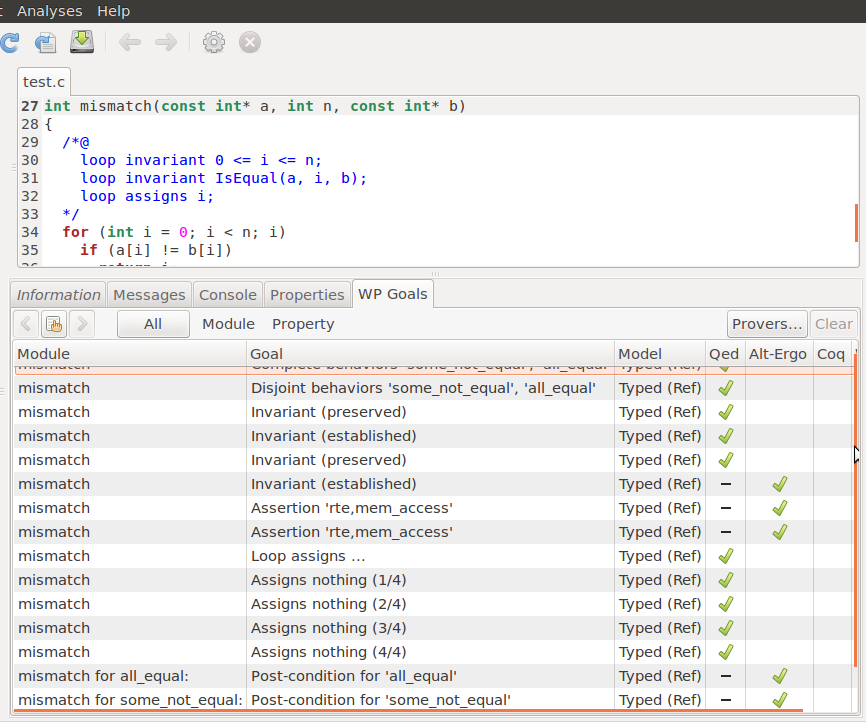
\includegraphics[width=0.9\textwidth]{images/frama-c-partial-correctness.png}
\caption{Frama-C beweist den Algorithmus trotz Tippfehler (\texttt{i} statt \texttt{i++})}
\end{figure}

Um solche Fehler zu vermeiden, muss die totale Korrektheit bewiesen werden. Dazu muss im Falle von Schleifen 
eine sogenannte Variante ergänzt werden, die in jeder Iteration kleiner wird und in endlich Schritten zu einem 
kleinstem Element führt (siehe dazu das Kapitel 2.2).

Beide Verifikationswerkzeuge erlauben die Notation und Verifizierung einer solchen Variante analog zur
Schleifeninvariante. Die folgende Schleife (aus der Implementierung von \texttt{equal}) wurde mit einer Variante 
in ACSL-Syntax angereichert. Die Notation in VeriFast unterscheidet sich nur darin, dass das einleitende
Schlüsselwort \texttt{decreases} lautet.

\lstinputlisting[language=C, caption=Schleifenvariante in ACSL]{codes/loop_variant_acsl.c}

Da der Nachweis der Terminierung aber nicht immer so einfach möglich ist, stellt die Kombination
der Verfizierung mit automatisch ausführbaren Modultests (engl. unit tests) eine sinnvolle Alternative bzw. Ergänzung dar.
Schon ein einziger Test würde ausreichen, um den Tippfehler aus dem Screenshot aufzudecken. 

In allen Fällen, in denen die Terminierung nur sehr schwierig oder gar nicht zu beweisen ist, bieten
Tests außerdem eine einfachere bzw. überhaupt eine Lösung. Auch wenn damit natürlich
kein Beweis der totalen Korrektheit zu erbringen ist.

ACSL kann darüber hinaus auch die Terminierung von rekursiven Funktionen prüfen, was in
VeriFast derzeit nicht möglich ist.


\section{Arithmetische Überläufe}
\label{sec:implementation:overflows}

Die beiden Werkzeuge können arithmetische Überläufe ganzer Zahlen erkennen, jedoch ist diese Überprüfung
optional\footnote{VeriFast: Die Überprüfung kann an der Oberfläche deaktiviert werden. Frama-C: Nur bei eingeschaltetem -rte Parameter.}.

Zum Nachweis der Abwesenheite von Überläufen muss im Kontrakt oder in entsprechenden Ghostbefehlen der Wertebereich
der Variablen entsprechend eingeschränkt werden. Für diesen Zweck liefert VeriFast entsprechende Lemmas
wie \lstinline{integer_limits} mit. Solange bei der Verifizierung jedoch kein Überlauf erkannt wird,
ist nicht einsehbar an welchen Stellen eine Prüfung stattfindet. Frama-C ist in diesem Fall
transparenter, jede potenzielle Stelle wird erkenntlich gemacht.


